\chapter{Software}

\section{Instalação do sistema}

Para a execução e instalação do software, necessita-se da execução de um \textit{workflow } de forma que a \textit{Build} e o \textit{Deploy} sejam executados com o Docker na Jetson.

Docker é uma tecnologia de conteinerização que serve para modularizar a sua aplicação, de forma que as dependências de cada bloco do software, seja executada de maneira independente, como em uma máquina virtual. 

Para construir uma imagem Docker na sua máquina:
\begin{itemize}
    \item Utilize o comando 'docker build --pull'
    \item Teste a imagem construída com o comando 'docker run -it nomedoconteiner'
    \item Executar o contêiner com o comando 'docker run'
\end{itemize}

\begin{figure}[H]
  \centering
  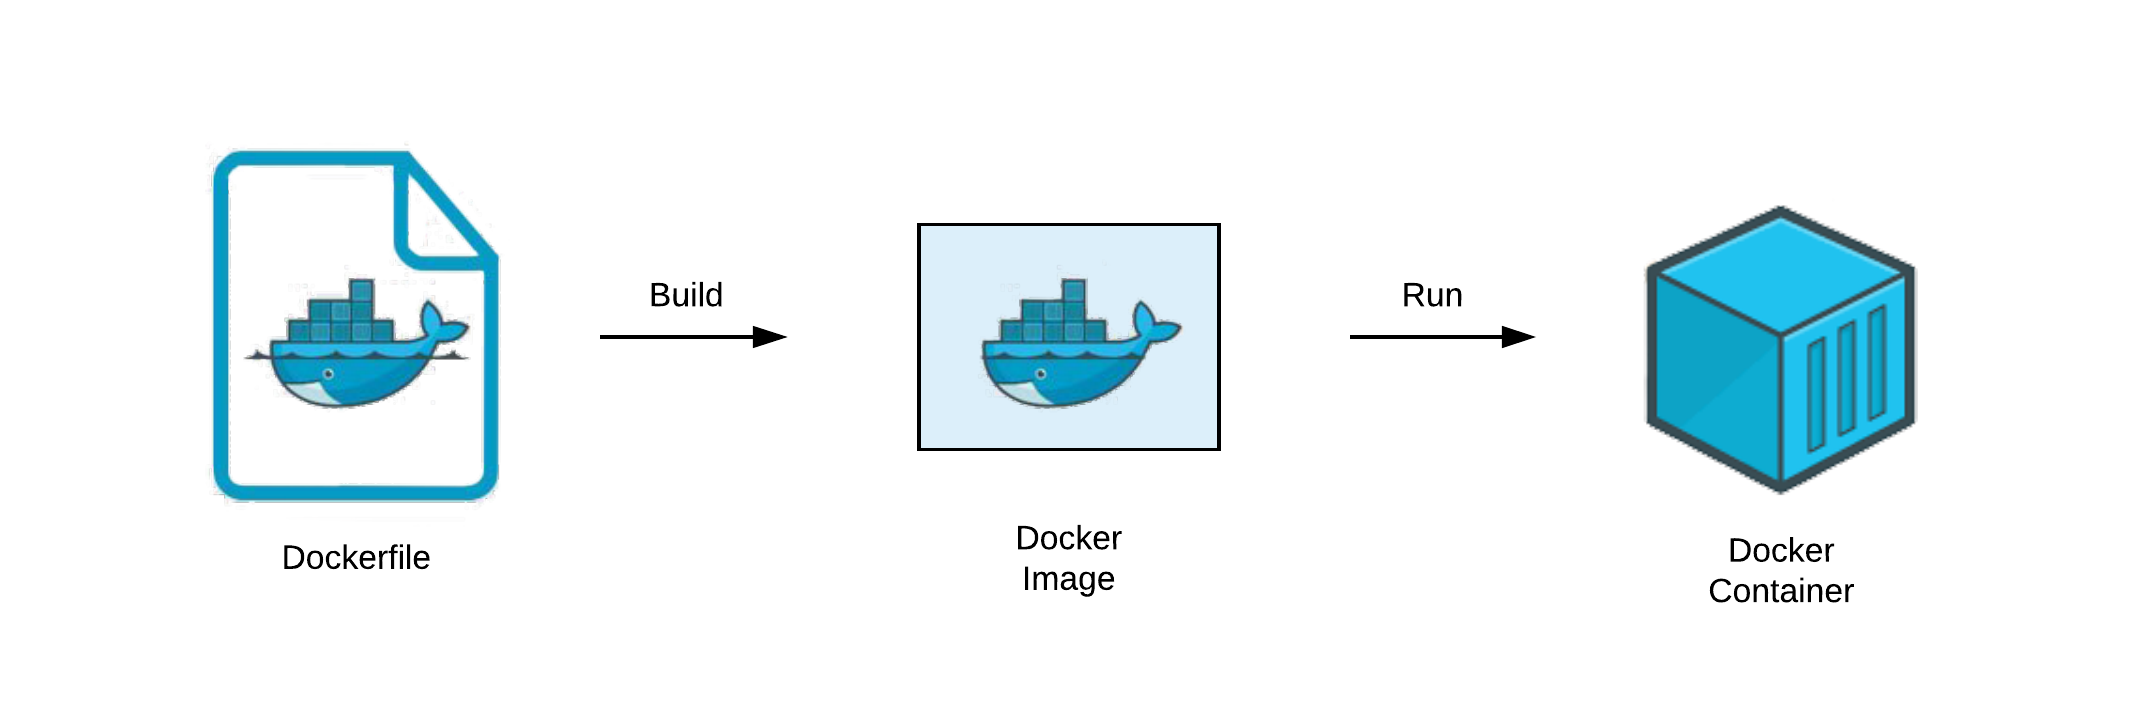
\includegraphics[keepaspectratio=true,scale=0.2] {Figuras/Software/dockerfiletocontainer.png}
  \caption{Pipeline de execução de comandos docker} 
 { \footnotesize FONTE: "www.docker.com".} 
  \label{fig:docker}
\end{figure}

\section{Atualização do Sistema}

As atualizações do software se darão por meio da atualização da imagem do Docker no repositório oficial do produto no Dockerhub. Para isso, deve-se atualizar a imagem utilizada pelo projeto por meio do comando 'docker pull '. Esse comando irá atualizar o ambiente em que a aplicação estará sendo executada.

\begin{figure}[H]
  \centering
  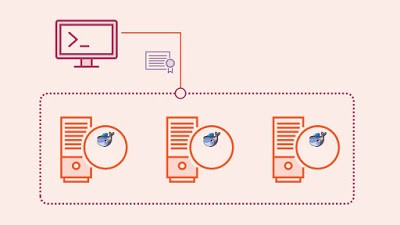
\includegraphics[keepaspectratio=true,scale=0.8] {Figuras/coneiner.jpg}
  \caption{Exemplo de conteiners docker simultâneos} 
 { \footnotesize FONTE: "www.docker.com".} 
  \label{fig:docker}
\end{figure}